\chapter{El supersespacio y la construcción de la dinámica supersimétrica}

\lectureoverview{Reconstruimos la supersimetría a partir del sistema más pequeño en el que puede actuar: un oscilador bosónico y otro fermiónico con la misma energía. El contraste entre sus ecuaciones de segundo y primer orden conduce a las cargas supersimétricas y a su álgebra. Después reinterpretamos esa álgebra como geometría en un espacio con la coordenada ordinaria (t) y las coordenadas de Grassmann \(\theta,\bar\theta\). Los supercampos reúnen los bosones, los fermiones y un campo auxiliar en un solo objeto; la integración de Berezin extrae un lagrangiano ordinario invariante; las derivadas covariantes permiten imponer restricciones compatibles con la simetría; y la restricción quiral ofrece el primer ejemplo importante. La lección muestra deliberadamente las dificultades de signos y ordenación de este formalismo y concluye explicando por qué la simetría misma es más fundamental que un catálogo de reglas de Feynman.}

\section{Volvamos al sistema de un modo}

Empecemos de nuevo con fermiones y bosones en reposo. Omitimos todas las coordenadas espaciales y las etiquetas de momento. En un modo dado, un cuanto está presente o ausente, y basta con los operadores de creación y aniquilación para describirlo. Escribamos \(a^\dagger,a\) para un modo bosónico y \(c^\dagger,c\) para uno fermiónico. Satisfacen
\begin{align}
[a,a^\dagger]&=1,
&
\{c,c^\dagger\}&=1,
&
c^2=(c^\dagger)^2&=0.
\end{align}
Si ambos cuantos tienen la misma energía \(m\), entonces, salvo una constante irrelevante del vacío,
\begin{equation}
H=m\left(a^\dagger a+c^\dagger c\right).
\label{eq:l7-one-mode-hamiltonian}
\end{equation}
El operador número \(a^\dagger a\) puede tomar cualquier valor entero no negativo, mientras que \(c^\dagger c\) solo puede valer cero o uno. Esta es toda la cinemática del modelo de juguete.

Esta simplificación es estratégica. Queremos entender la operación que elimina un bosón e introduce un fermión, o hace lo contrario, sin cambiar la energía. Sin embargo, antes de construir esa operación, traduciremos el mismo sistema del lenguaje de operadores al lenguaje lagrangiano.

\section{El oscilador bosónico}

Para el bosón, introduzcamos una coordenada real \(\phi(t)\). Sin variación espacial, un campo escalar libre se convierte en un oscilador armónico ordinario. La primera expresión que se escribió en la pizarra fue
\[
\frac{1}{2}\dot\phi^{,2}+\frac{1}{2}m^2\phi^2.
\]
Esa expresión es la energía cinética más la potencial, no el lagrangiano. En la lección se corrige inmediatamente el signo:
\begin{equation}
L_B=\frac{1}{2}\dot\phi^{,2}-\frac{1}{2}m^2\phi^2.
\label{eq:l7-boson-lagrangian}
\end{equation}

\begin{figure}[H]
\centering
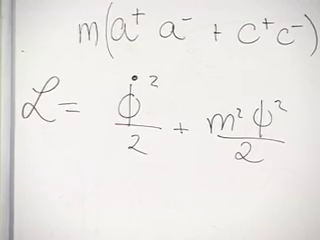
\includegraphics[width=0.62\textwidth]{lecture_07_figure_02.png}
\lectureframe{00:03:25.431}
\caption{El hamiltoniano de un modo aparece sobre el lagrangiano bosónico. La imagen conserva el signo más inicial antes de la corrección verbal a \(T-V\).}
\end{figure}

\begin{classroomqa}
\audiencequestion{¿Qué tiene de incorrecto el signo del lagrangiano del oscilador que aparece en la ecuación? \lecturetimestamp{00:04:00}}
\lecturerresponse{La energía es \(T+V\), pero el lagrangiano es \(T-V\). Por tanto, el término de potencial debe llevar un signo menos. La corrección cambia la ecuación, que pasa de describir un comportamiento exponencial a la oscilación armónica esperada.}
\end{classroomqa}

En efecto, la ecuación de Euler--Lagrange da
\begin{align}
\frac{d}{dt}\frac{\partial L_B}{\partial\dot\phi}
&=\frac{\partial L_B}{\partial\phi},\\
\ddot\phi&=-m^2\phi,
\end{align}
o bien
\begin{equation}
\ddot\phi+m^2\phi=0.
\label{eq:l7-boson-eom}
\end{equation}
Su frecuencia es \(m\), no \(m^2\). La cuantización de este oscilador produce la misma sucesión de estados descrita por \(a^\dagger\) y \(a\) en la ecuación ~\eqref{eq:l7-one-mode-hamiltonian}.

\section{Por qué la acción fermiónica es de primer orden}

El lagrangiano fermiónico parece más sencillo porque contiene una sola derivada temporal. La razón ya se aprecia en un intento deliberadamente ingenuo. Para una variable conmutativa ordinaria,
\begin{equation}
L_{\mathrm{trial}}=\phi\dot\phi
=\frac{1}{2}\frac{d}{dt}\phi^2.
\end{equation}
Es una derivada total. Su ecuación de Euler--Lagrange solo dice que \(\dot\phi=\dot\phi\), así que cualquier trayectoria diferenciable está permitida. Eliminar una derivada total de la acción cambia los datos de los extremos, pero no la ecuación de movimiento en el interior.

Ahora llamemos \(\psi\) a la variable y declarémosla impar de Grassmann. Tanto \(\psi\) como \(\dot\psi\) anticonmutan. Si se elige fijar la variación por la izquierda, reordenar los factores impares introduce un signo menos, de modo que el mismo intento formal da
\begin{equation}
\frac{d}{dt}\frac{\partial L_{\mathrm{trial}}}{\partial\dot\psi}
=\dot\psi,
\qquad
\frac{\partial L_{\mathrm{trial}}}{\partial\psi}
=-\dot\psi.
\end{equation}
Por tanto, la ecuación es
\begin{equation}
\dot\psi=-\dot\psi
\quad\Longrightarrow\quad
\dot\psi=0.
\label{eq:l7-constant-fermion}
\end{equation}
La expresión que era una tautología para una coordenada conmutativa adquiere contenido dinámico para una variable anticonmutativa. Contiene demasiado para un oscilador, pues solo permite una constante, pero precisamente ahí está la pista que necesitamos.

\begin{classroomqa}
\audiencequestion{¿La solución es simplemente que \(\psi\) es constante? \lecturetimestamp{00:13:57}}
\lecturerresponse{Sí. La ecuación~\eqref{eq:l7-constant-fermion} es una ecuación diferencial genuina de primer orden, cuya solución es una constante arbitraria con valores de Grassmann. Un término de masa convertirá esa solución estática en una oscilante.}
\end{classroomqa}

El intento obvio, \(m\psi^2\), falla porque \(\psi^2=0\). Necesitamos dos variables reales impares \(\psi_1,\psi_2\), o, de manera equivalente, una variable compleja y su conjugada. En la lección se desarrolla en la pizarra la formulación con dos variables reales, revisando una y otra vez los signos y los factores de dos. Una formulación compleja con normalización convencional es
\begin{equation}
L_F=\frac{i}{2}
\left(\bar\psi\dot\psi-\dot{\bar\psi}\psi\right)
-m\bar\psi\psi.
\label{eq:l7-fermion-lagrangian}
\end{equation}
Salvo una derivada total, esto es \(i\bar\psi\dot\psi-m\bar\psi\psi\). Al variar \(\bar\psi\) se obtiene
\begin{equation}
i\dot\psi=m\psi,
\qquad
\psi(t)=\psi(0)e^{-imt}.
\label{eq:l7-fermion-eom}
\end{equation}
La ecuación conjugada tiene la fase opuesta. Así, el modo fermiónico oscila con energía \(m\), igual que el bosónico, aunque su ecuación sea de primer orden en vez de segundo.

\editorialnote{~\eqref{eq:l7-fermion-lagrangian} fija una ordenación y normalización estándar para el cálculo exploratorio con dos variables reales. En la lección se introduce el factor \(i\), se ajusta un factor de dos y queda sin resolver el signo de una componente real. Estos cambios no alteran la conclusión central: la cinética fermiónica es de primer orden, la masa aparece linealmente y un fermión complejo proporciona un bilineal no nulo.}

Esta es la versión en dimensión cero de un contraste relativista conocido. La ecuación de Klein--Gordon es de segundo orden en el tiempo, mientras que la ecuación de Dirac es de primer orden. Al suprimir el espacio, el bosón se convierte en un oscilador armónico y el fermión en un oscilador complejo de Grassmann.

\begin{classroomqa}
\audiencequestion{¿Importa el orden en que se escriben \(\psi\), \(\dot\psi\) y sus conjugadas? \lecturetimestamp{00:18:58}}
\lecturerresponse{Las fórmulas intermedias sí dependen del orden, porque los factores impares anticonmutan. La teoría física no depende de una preferencia arbitraria al escribir, siempre que se emplee de manera coherente una misma convención para la variación por la izquierda o por la derecha, la conjugación y la integración. Invertir un par de factores impares cambia un signo, y ese signo debe cambiarse también en todo lo demás de manera coherente.}
\end{classroomqa}

Al combinar las ecuaciones ~\eqref{eq:l7-boson-lagrangian} y \eqref{eq:l7-fermion-lagrangian} obtenemos una descripción lagrangiana del mismo par degenerado representado por la ecuación ~\eqref{eq:l7-one-mode-hamiltonian}. Ya podemos identificar la simetría que los relaciona.

\section{Las cargas supersimétricas y su álgebra}

Un operador que elimina un fermión e introduce un bosón es
\begin{equation}
Q^\dagger=\sqrt{2m}\,a^\dagger c,
\end{equation}
mientras que su conjugado elimina un bosón e introduce un fermión,
\begin{equation}
Q=\sqrt{2m}\,a c^\dagger.
\end{equation}
La normalización se elige para que el álgebra adopte su forma estándar. Usando \(cc^\dagger=1-c^\dagger c\), \(aa^\dagger=a^\dagger a+1\) y el hecho de que los operadores bosónicos conmutan con los fermiónicos,
\begin{align}
\{Q,Q^\dagger\}
&=2m\left(ac^\dagger a^\dagger c+a^\dagger c a c^\dagger\right)\notag\\
&=2m\left[(a^\dagger a+1)c^\dagger c
+a^\dagger a(1-c^\dagger c)\right]\notag\\
&=2m\left(a^\dagger a+c^\dagger c\right)=2H.
\label{eq:l7-superalgebra}
\end{align}
Los operadores bosónicos pueden desplazarse a través de los fermiónicos. La misma nilpotencia que limita la ocupación fermiónica implica
\begin{equation}
Q^2=(Q^\dagger)^2=0.
\end{equation}
Por último,
\begin{equation}
[H,Q]=[H,Q^\dagger]=0.
\label{eq:l7-conserved-supercharges}
\end{equation}
Cada carga supersimétrica cambia el número de bosones y el de fermiones en sentidos opuestos, así que los dos cambios de energía se cancelan cuando las frecuencias son iguales.

\begin{classroomqa}
\audiencequestion{¿Qué es \([H,Q]\)? ¿La respuesta es proporcional a \(Q\)? \lecturetimestamp{00:25:10}}
\lecturerresponse{No. La respuesta es cero. Un operador de creación o aniquilación aislado adquiriría la energía correspondiente al conmutar con \(H\), pero las contribuciones bosónica y fermiónica en \(Q\) se cancelan. Esa cancelación se debe precisamente a la condición de igualdad de energías.}
\end{classroomqa}

\begin{classroomqa}
\audiencequestion{¿No se había escrito ya ese conmutador en la pizarra? \lecturetimestamp{00:25:45}}
\lecturerresponse{Sí. Volver a encontrarlo es útil porque nos obliga a interpretar la relación en vez de limitarnos a copiarla: conmutar con el hamiltoniano significa que la transformación es una simetría y que su generador se conserva.}
\end{classroomqa}

El adjetivo \emph{carga} alude a esta ley de conservación. Sin embargo, no debemos tratar \(Q\) como un número ordinario que pueda medirse simultáneamente y que esté asociado a un estado. Es impar de Grassmann, nilpotente y transforma un estado bosónico en uno fermiónico. Lo útil es afirmar que es un generador conservado que actúa dentro de supermultipletes degenerados.
\editorialnote{Esta formulación precisa la analogía de clase que consiste en etiquetar los estados por su energía o su carga eléctrica. Las cargas supersimétricas impares individuales no hermíticas no son observables ordinarios que tengan números cuánticos numéricos. La acción conservada de estas cargas y la representación del superálgebra completo proporcionan la clasificación adecuada.}

\section{Los generadores como derivadas}

El álgebra es compacta, pero por sí sola no nos dice cómo construir teorías con interacciones. El siguiente paso es geométrico. Los generadores de simetrías conocidos ya actúan como operadores diferenciales. Según la convención de la lección,
\begin{equation}
H=i\frac{\partial}{\partial t},
\qquad
P=-i\frac{\partial}{\partial x}.
\end{equation}

\begin{figure}[H]
\centering
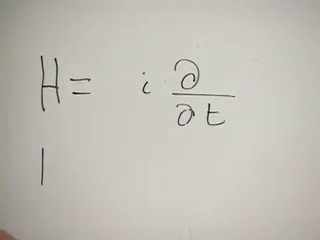
\includegraphics[width=0.50\textwidth]{lecture_07_figure_03.png}
\lectureframe{00:28:12.720}
\caption{El hamiltoniano representado como generador de las traslaciones temporales.}
\end{figure}

El momento angular también es una coordenada multiplicada por una derivada. Si las cargas supersimétricas son generadores impares, cabe preguntarse si pueden representarse mediante derivadas respecto de coordenadas impares. Por ello, ampliamos el eje temporal al supersespacio
\begin{equation}
(t,\theta,\bar\theta),
\qquad
\theta^2=\bar\theta^2=0,
\qquad
\theta\bar\theta=-\bar\theta\theta.
\end{equation}
Los campos en este espacio dependen de un tiempo ordinario y de un par conjugado de coordenadas de Grassmann.

La lección muestra deliberadamente cuán traicioneros pueden ser los signos. El signo debido a la conjugación compleja, el que aparece al mover un parámetro impar y el que resulta de elegir derivadas por la izquierda en vez de por la derecha corresponden a operaciones distintas. En lugar de conservar etapas incompatibles de la pizarra, fijaremos ahora una convención: todas las derivadas impares son por la izquierda, y
\begin{equation}
q=\partial_\theta+i\bar\theta\partial_t,
\qquad
\bar q=\partial_{\bar\theta}+i\theta\partial_t.
\label{eq:l7-differential-supercharges}
\end{equation}
Entonces
\begin{equation}
q^2=\bar q^{,2}=0,
\qquad
\{q,\bar q\}=2i\partial_t=2H.
\label{eq:l7-differential-algebra}
\end{equation}
El factor de dos procede de dos términos cruzados: \(\{\partial_\theta,\theta\}=1\) y \(\{\partial_{\bar\theta},\bar\theta\}=1\). Si los generadores solo contuvieran \(\partial_\theta\) y \(\partial_{\bar\theta}\), su anticonmutador se anularía y no podría reproducir el hamiltoniano.

\begin{classroomqa}
\audiencequestion{¿Deben llevar el mismo signo los dos términos con derivadas temporales en \(q\) y \(\bar q\)? \lecturetimestamp{00:31:01}}
\lecturerresponse{Hay que elegirlos de forma coherente para que el anticonmutador mixto sea \(2H\). Se puede usar una convención global con signo más o su alternativa conjugada coherente. El cálculo, y no la intuición visual sobre el símbolo \(i\), determina los signos relativos.}
\end{classroomqa}

En la sala se revisan los signos una y otra vez, y la dificultad acaba convirtiéndose en una broma: parece que los signos cambian durante el trayecto al trabajo. La broma viene al caso. Al hacer pasar un parámetro de Grassmann a través de una coordenada puede cambiar un signo, aunque no haya cambiado ninguna convención física. La ecuación~\eqref{eq:l7-differential-supercharges} es la referencia fija para todo lo que sigue.

\subsection{La supersimetría como desplazamiento de coordenadas}

Sean \(\xi,\bar\xi\) parámetros infinitesimales impares. La acción sobre un supercampo mediante
\begin{equation}
\delta_\xi=\xi q+\bar\xi\bar q
\end{equation}
equivale, según la convención anterior, al cambio infinitesimal de coordenadas
\begin{align}
\theta&\longrightarrow\theta+\xi,\\
\bar\theta&\longrightarrow\bar\theta+\bar\xi,\\
t&\longrightarrow t+i\left(\xi\bar\theta+\bar\xi\theta\right).
\label{eq:l7-coordinate-shift}
\end{align}
Por tanto, la variación de un supercampo escalar es
\begin{equation}
\delta_\xi\Phi
=\left(\xi\partial_\theta+\bar\xi\partial_{\bar\theta}
+i\xi\bar\theta\partial_t+i\bar\xi\theta\partial_t\right)\Phi
=\left(\xi q+\bar\xi\bar q\right)\Phi.
\end{equation}
Este es el contenido geométrico de la supersimetría. Es una traslación en direcciones impares ligada a una traslación en el tiempo ordinario. Dos desplazamientos impares se cierran en una traslación temporal, de acuerdo con la ecuación~\eqref{eq:l7-differential-algebra}.

\begin{classroomqa}
\audiencequestion{¿Podría el signo menos en disputa representar un movimiento hacia atrás en el tiempo? \lecturetimestamp{00:58:13}}
\lecturerresponse{Una convención distinta para los signos puede invertir el desplazamiento temporal infinitesimal que se muestra, pero no introduce ningún proceso físico separado de retroceso temporal. Lo que importa es que la transformación de coordenadas y los generadores diferenciales obedezcan la misma álgebra.}
\end{classroomqa}

\begin{classroomqa}
\audiencequestion{¿Tiene este tiempo extendido una realización física o es solo un artificio formal? \lecturetimestamp{00:58:23}}
\lecturerresponse{En cierto sentido útil, es un artificio formal: organiza el álgebra en una estructura geométrica. Pero esta estructura resulta físicamente valiosa al introducir interacciones. El supersespacio proporciona un cálculo sistemático para construir lagrangianos que preservan la simetría entre bosones y fermiones--en cada paso, del mismo modo que el cálculo tensorial ayuda a construir escalares de Lorentz.}
\end{classroomqa}

\section{Supercampos y la componente auxiliar}

Como solo hay dos coordenadas impares, el desarrollo de un supercampo par termina:
\begin{equation}
\Phi(t,\theta,\bar\theta)
=\phi(t)+\bar\theta\psi(t)+\bar\psi(t)\theta
+D(t)\bar\theta\theta.
\label{eq:l7-superfield}
\end{equation}
Los coeficientes de los monomios pares, \(\phi\) y \(D\), son bosónicos; los coeficientes de los monomios impares, \(\psi\) y \(\bar\psi\), son fermiónicos. No sobrevive ningún término \(\theta^2\), \(\bar\theta^2\) ni de orden superior. Dejamos sin desarrollar la dependencia temporal, porque una serie de Taylor ordinaria en \(t\) no terminaría y aquí no serviría de nada.

\begin{classroomqa}
\audiencequestion{¿Qué representa la componente \(D(t)\) del término de orden superior? \lecturetimestamp{00:41:46}}
\lecturerresponse{En esta etapa es simplemente el coeficiente bosónico final del desarrollo finito. En la acción por componentes normalmente no tiene término cinético y se elimina mediante una ecuación de movimiento algebraica; por eso se llama campo auxiliar. En tono jocoso, la lección sugiere ``D de «dummy»,'' que expresa su papel no dinámico, aunque esa no sea la definición histórica.}
\end{classroomqa}

El supercampo es un solo objeto, mientras que \(\phi,\psi,\bar\psi,D\) son sus componentes. Una transformación supersimétrica los mezcla. Así, un bosón y un fermión están relacionados de una manera estructural muy parecida a la relación entre las componentes \(x\) y \(y\) de un vector bajo una rotación, aunque las direcciones de Grassmann no puedan representarse como ejes ordinarios.

\section{La superacción y la componente de orden superior}

Para obtener ecuaciones de movimiento necesitamos una acción. En teoría de campos ordinaria se forma un lagrangiano escalar y se integra sobre el espacio-tiempo. Aquí, la expresión análoga es
\begin{equation}
S=\int dt\,d\theta\,d\bar\theta\;\Lambda
\bigl(\Phi,\text{ superspace derivatives of }\Phi\bigr),
\label{eq:l7-superaction}
\end{equation}
donde \(\Lambda\) es un supercampo par. La integración de Berezin es algebraica. Elegimos
\begin{equation}
\int d\theta\,d\bar\theta\;\bar\theta\theta=1.
\end{equation}
Por tanto, si
\begin{equation}
\Lambda=A+\bar\theta B+\bar B\theta+C\bar\theta\theta,
\end{equation}
entonces
\begin{equation}
\int d\theta\,d\bar\theta\;\Lambda=C.
\label{eq:l7-top-component}
\end{equation}
La integración respecto de las coordenadas impares extrae la componente de orden superior y deja un lagrangiano ordinario que se integra respecto del tiempo.

¿Por qué es invariante el resultado? Una variación supersimétrica traslada las variables de integración. La variación de la componente de orden superior es una derivada total ordinaria respecto del tiempo, mientras que las derivadas totales impares se anulan al integrar según Berezin. Con condiciones adecuadas en los extremos, la acción no cambia. Este es el análogo en el supersespacio de construir un escalar de Lorentz antes de integrarlo sobre el espacio-tiempo.

\section{Producto de supercampos}

La manera más sencilla de obtener un supercampo nuevo a partir de uno dado es multiplicarlo por sí mismo. Partiendo de la ecuación~\eqref{eq:l7-superfield}, se anula todo término que contenga \(\theta^2\) o \(\bar\theta^2\). Manteniendo el orden \(\bar\theta\theta\) y colocando a la izquierda los campos componentes con barra, obtenemos
\begin{align}
\Phi^2
={}&\phi^2
+2\phi\bar\theta\psi
+2\phi\bar\psi\theta\notag\\
&+\left(2\phi D-2\bar\psi\psi\right)\bar\theta\theta.
\label{eq:l7-superfield-square}
\end{align}

\begin{figure}[H]
\centering
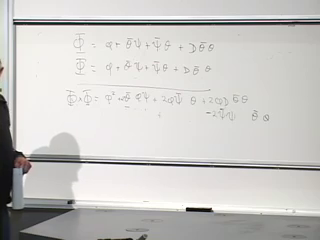
\includegraphics[width=0.82\textwidth]{lecture_07_figure_05.png}
\lectureframe{01:07:57.844}
\caption{El producto de supercampos componente a componente y la colección de sus términos \(\bar\theta\theta\).}
\end{figure}

Los dos términos \(\phi D\) y \(D\phi\) se suman porque ambos campos son pares. Los dos términos cruzados fermiónicos también se suman después de reordenar cada uno, pero ambos llevan el mismo signo negativo:
\begin{equation}
(\bar\theta\psi)(\bar\psi\theta)
+(\bar\psi\theta)(\bar\theta\psi)
=-2\bar\psi\psi\,\bar\theta\theta.
\end{equation}
Al integrar el cuadrado respecto de las coordenadas impares se obtiene
\begin{equation}
\int d\theta\,d\bar\theta\;\Phi^2
=2\phi D-2\bar\psi\psi.
\end{equation}
Este término es supersimétrico por construcción, pero aún no es un lagrangiano cinético. No contiene derivadas temporales.

A continuación, en la pizarra se proponen \(\Phi^3\), \(\Phi^4\) y \(\Phi^n\) como ejercicios. Hay una regla compacta. Para cualquier función ordinaria \(W\),
\begin{equation}
\left.W(\Phi)\right|_{\bar\theta\theta}
=W'(\phi)D-W''(\phi)\bar\psi\psi.
\label{eq:l7-function-top-component}
\end{equation}
Para \(W(\phi)=\phi^2\), esto reproduce la ecuación~\eqref{eq:l7-superfield-square}; para \(W(\phi)=\phi^n\), da
\begin{equation}
\left.\Phi^n\right|_{\bar\theta\theta}
=n\phi^{n-1}D-n(n-1)\phi^{n-2}\bar\psi\psi.
\end{equation}
\editorialnote{La lección propone como ejercicio la potencia \(n\) y anticipa qué tipos de términos cabe esperar. La ecuación~\eqref{eq:l7-function-top-component} proporciona la regla completa con la convención de orden fijada.}

En este punto, el profesor pregunta si el público está agotado. El público responde que no; él contesta que sí lo está. El intercambio es algo más que un alivio cómico. Las potencias de supercampos son fáciles porque el desarrollo termina, pero las derivadas y las restricciones son donde la contabilidad de signos se vuelve realmente exigente.

\section{¿Qué derivadas respetan la supersimetría?}

Antes de seguir el siguiente argumento de la pizarra, hay que hacer una corrección. La derivada temporal ordinaria no plantea ningún problema:
\begin{equation}
[\partial_t,q]=[\partial_t,\bar q]=0.
\end{equation}
Por consiguiente, \(\partial_t\Phi\) se transforma como un supercampo siempre que lo haga \(\Phi\). Los objetos sutiles son las derivadas impares sin modificar \(\partial_\theta\Phi\) y \(\partial_{\bar\theta}\Phi\), porque no anticonmutan con ambas cargas supersimétricas. Necesitamos derivadas impares modificadas para las restricciones y para construir componentes de manera manifiestamente supersimétrica.
\editorialnote{La afirmación verbal de que la derivación temporal no produce otro supercampo no es correcta con la convención que usamos aquí. Como \(\partial_t\) conmuta con ambas cargas supersimétricas, es covariante. La construcción posterior de derivadas impares modificadas sigue siendo necesaria y constituye el verdadero punto matemático de la lección.}

\subsection{La analogía del campo «mágico»``''}

La lección motiva el criterio mediante rotaciones ordinarias. Sea \(f(x,y)\) tal que
\begin{equation}
\partial_y f=0.
\label{eq:l7-magic-constraint}
\end{equation}
Llamemos a una función así campo ``«mágico».'' Depende de \(x\), pero no de \(y\). ¿Se conserva la clase de campos mágicos bajo rotaciones? Para
\begin{equation}
L_z=-i\left(x\partial_y-y\partial_x\right),
\end{equation}
obtenemos
\begin{equation}
[\partial_y,L_z]=i\partial_x\neq0.
\end{equation}
Por tanto, \(L_z f\) en general adquiere dependencia respecto de \(y\), aunque \(f\) satisfaga inicialmente la ecuación~\eqref{eq:l7-magic-constraint}. La restricción no es invariante bajo rotaciones.

La lección general es sencilla. Si un campo satisface \(C\Phi=0\) y una simetría está generada por \(G\), el campo transformado sigue satisfaciendo la restricción cuando el conmutador graduado de \(C\) y \(G\) se anula. Para dos operadores impares, el conmutador graduado es un anticonmutador.

\begin{classroomqa}
\audiencequestion{¿Cuándo es compatible con una simetría una restricción impuesta a un campo? \lecturetimestamp{01:17:56}}
\lecturerresponse{Cuando el operador de restricción conmuta en sentido graduado con los generadores de simetría. Entonces se puede desplazar \(C(G\Phi)\) a través de \(G\) y reducirlo a \(G(C\Phi)=0\). El ejemplo de la rotación falla porque \(\partial_y\) no conmuta con el generador de rotaciones.}
\end{classroomqa}

\subsection{Derivadas impares covariantes}

Con las cargas supersimétricas fijadas por la ecuación~\eqref{eq:l7-differential-supercharges}, definimos
\begin{equation}
\mathcal D=\partial_\theta-i\bar\theta\partial_t,
\qquad
\bar{\mathcal D}=\partial_{\bar\theta}-i\theta\partial_t.
\label{eq:l7-covariant-derivatives}
\end{equation}
El único cambio es el signo del término con derivada temporal. El cálculo directo da
\begin{align}
\{\mathcal D,q\}
&=\{\mathcal D,\bar q\}
=\{\bar{\mathcal D},q\}
=\{\bar{\mathcal D},\bar q\}=0,\\
\{\mathcal D,\bar{\mathcal D}\}&=-2i\partial_t.
\label{eq:l7-covariant-algebra}
\end{align}
Los dos términos cruzados potencialmente no nulos se cancelan. Es el análogo impar de una derivada covariante: deriva preservando la ley de transformación.

En la lección se usa \(D\) tanto para la componente auxiliar como para esta derivada. Reservamos \(D(t)\) para la componente y usamos la letra caligráfica \(\mathcal D\) para el operador.

\section{La restricción quiral}

Ahora podemos imponer una restricción no trivial que se conserva bajo la supersimetría:
\begin{equation}
\bar{\mathcal D}\Phi=0.
\label{eq:l7-chiral-constraint}
\end{equation}
Un campo que la satisface se llama quiral. Si es quiral antes de una transformación supersimétrica, entonces
\begin{equation}
\bar{\mathcal D}(q\Phi)
=-q(\bar{\mathcal D}\Phi)=0,
\qquad
\bar{\mathcal D}(\bar q\Phi)
=-\bar q(\bar{\mathcal D}\Phi)=0.
\end{equation}
Así, el supercampo transformado entero permanece dentro de la clase restringida. A diferencia de la condición de campo mágico, la quiralidad es compatible con la simetría.

Para resolver la restricción, definimos una coordenada temporal desplazada
\begin{equation}
\tau=t+i\bar\theta\theta.
\label{eq:l7-chiral-time}
\end{equation}
Como usamos derivadas por la izquierda,
\begin{equation}
\partial_{\bar\theta}\tau=i\theta,
\end{equation}
y, por tanto,
\begin{equation}
\bar{\mathcal D}F(\tau,\theta)
=\left(\partial_{\bar\theta}-i\theta\partial_t\right)F(\tau,\theta)
=i\theta\partial_\tau F-i\theta\partial_\tau F=0.
\end{equation}
Así pues, el supercampo quiral local más general depende de \(\bar\theta\) solo a través de \(\tau\):
\begin{equation}
\Phi_{\mathrm{ch}}(\tau,\theta)
=\phi(\tau)+\bar\psi(\tau)\theta.
\label{eq:l7-chiral-field-tau}
\end{equation}

\begin{classroomqa}
\audiencequestion{¿Depender de \(\tau\) y \(\theta\) es la única forma de satisfacer la restricción quiral? \lecturetimestamp{01:32:35}}
\lecturerresponse{Localmente, sí. La ecuación diferencial \(\bar{\mathcal D}\Phi=0\) dice precisamente que la dependencia independiente respecto de \(\bar\theta\) puede incorporarse a la coordenada desplazada \(\tau=t+i\bar\theta\theta\). El desarrollo finito restante es una función de \(\tau\) más un término proporcional a \(\theta\).}
\end{classroomqa}

Al volver a desarrollar en la coordenada temporal original,
\begin{align}
\phi(\tau)
&=\phi(t)+i\bar\theta\theta\dot\phi(t),\\
\bar\psi(\tau)\theta
&=\bar\psi(t)\theta,
\end{align}
pues la corrección a la segunda línea contiene \(\theta^2\). Así,
\begin{equation}
\Phi_{\mathrm{ch}}(t,\theta,\bar\theta)
=\phi(t)+\bar\psi(t)\theta
+i\bar\theta\theta\dot\phi(t).
\label{eq:l7-chiral-field-components}
\end{equation}

\begin{classroomqa}
\audiencequestion{¿Debe incluir un término de segundo orden el desarrollo de Taylor de \(\phi(t+i\bar\theta\theta)\)? \lecturetimestamp{01:33:51}}
\lecturerresponse{No. La primera corrección es \(i\bar\theta\theta\dot\phi\), y todas las correcciones de orden superior contienen \((\bar\theta\theta)^2=0\). El público lo advierte enseguida: la nilpotencia ya había dado los dos primeros términos y había truncado la serie.}
\end{classroomqa}

Esta es la economía de la quiralidad. El supercampo sin restricciones de la ecuación~\eqref{eq:l7-superfield} tiene dos componentes bosónicas y dos fermiónicas. En este ejemplo mínimo unidimensional, la condición quiral elimina la componente auxiliar independiente y relaciona la componente de orden superior con \(\dot\phi\).

\section{El cálculo que, con razón, se interrumpe}

El siguiente paso natural es combinar el campo quiral con su conjugado e integrar en el supersespacio. Se empieza a escribir el desarrollo conjugado, y alguien del público pregunta si el orden \(\theta\bar\theta\) debe invertirse al conjugar. En ese momento, los signos dejan de parecer fiables. En vez de fingir seguridad, se interrumpe el cálculo.

\begin{classroomqa}
\audiencequestion{¿Podemos conocer el resultado principal aunque se posponga la multiplicación por el campo conjugado? \lecturetimestamp{01:37:30}}
\lecturerresponse{Sí. Si se tratan de manera coherente los signos y las conjugaciones, una expresión en el supersespacio construida a partir de un campo quiral y su conjugado produce los términos cinéticos bosónico y fermiónico ordinarios deseados. El resultado importante de esta lección es el principio de construcción, no una línea final poco fiable copiada de un cálculo hecho con cansancio.}
\end{classroomqa}

Conviene dejar visible el punto en que se interrumpe el cálculo. El formalismo no perdona: basta colocar mal un factor impar para cambiar un signo, y hay que conservar la misma convención al conjugar, derivar, multiplicar e integrar. Si se pierde esa coherencia, lo correcto es restablecerla antes de continuar. En una convención estándar, la acción cinética conocida se construye a partir de un producto con el campo conjugado, pero su reducción detallada por componentes corresponde al siguiente cálculo, hecho con cuidado, no a una reconstrucción de una línea inacabada de la pizarra.

\section{Por qué la simetría es la idea central}

Un lagrangiano supersimétrico hace más que colocar un bosón junto a un fermión. Restringe sus masas e interacciones para que formen una representación del superálgebra. En un vacío exactamente supersimétrico, los miembros de un supermultiplete tienen masas iguales. Sus contribuciones de lazos están correlacionadas, y los efectos ultravioleta bosónicos y fermiónicos se cancelan precisamente en las combinaciones impuestas por la simetría.

Por eso importa el aparato de construcción. Se podrían enumerar los vértices de Feynman y verificar las cancelaciones diagrama por diagrama, pero entonces estas parecerían accidentales. La supersimetría las explica del mismo modo que la simetría de Lorentz explica por qué las amplitudes de dispersión se transforman coherentemente en todos los sistemas de referencia inerciales.

\editorialnote{La supersimetría exacta no implica que se anule cada corrección individual a la autoenergía. Relaciona las renormalizaciones y elimina ciertas sensibilidades ultravioletas; los enunciados de no renormalización dependen de la magnitud, la dimensión y la cantidad de supersimetría. Se conserva aquí la afirmación amplia de la lección sobre las cancelaciones, expresada con estas salvedades.}

\begin{classroomqa}
\audiencequestion{¿Cómo se escribe ``«quiral»''? \lecturetimestamp{01:39:48}}
\lecturerresponse{Q-U-I-R-A-L. La palabra designa la restricción \(\bar{\mathcal D}\Phi=0\); no se refiere a la quiralidad geométrica ordinaria de un objeto en el espacio tridimensional, aunque la terminología provenga de la estructura levógira y dextrógira de los espinores relativistas.}
\end{classroomqa}

\begin{classroomqa}
\audiencequestion{¿Se podría prescindir del lagrangiano e ir directamente a las reglas de Feynman supersimétricas? \lecturetimestamp{01:40:00}}
\lecturerresponse{Desde luego, se pueden enunciar las reglas, pero entonces las relaciones entre los acoplamientos y las cancelaciones que producen parecen coincidencias sin explicación. El contenido más profundo es la simetría del espacio-tiempo generalizada. El lagrangiano, o una formulación invariante equivalente, hace visible esa razón y genera las reglas de forma sistemática.}
\end{classroomqa}

Supongamos que todos los órdenes perturbativos dieran amplitudes invariantes de Lorentz, aunque no se hubiera mencionado ninguna transformación de Lorentz. Tras suficientes cálculos, exigiríamos una explicación. La respuesta sería la simetría del espacio-tiempo que organiza de una vez todos los órdenes. El papel del superspacio es análogo: los desplazamientos en \(\theta,\bar\theta\) mezclan componentes bosónicas y fermiónicas, y su álgebra se cierra sobre las traslaciones en el espacio-tiempo.

\begin{classroomqa}
\audiencequestion{¿También habría que desarrollar las coordenadas espaciales ordinarias en una serie de potencias finita, como se hace con las coordenadas de Grassmann? \lecturetimestamp{01:44:55}}
\lecturerresponse{No. Una serie de potencias de una coordenada ordinaria no termina y, por lo general, no es la descomposición natural. Una transformada de Fourier resulta más útil porque descompone un campo en ondas y momentos. El desarrollo en \(\theta\) es especial precisamente porque la nilpotencia lo hace finito.}
\end{classroomqa}

\begin{classroomqa}
\audiencequestion{Si apareciera una partícula nueva en el LHC, ¿cómo podríamos saber si es una supercompañera y no simplemente una partícula desconocida? \lecturetimestamp{01:45:42}}
\lecturerresponse{La supersimetría predice números cuánticos e interacciones correlacionados, no solo un estado adicional. Los espines difieren en una unidad de un medio, las cargas gauge están relacionadas y muchos acoplamientos cúbicos y cuárticos dependen de menos parámetros independientes que en una teoría genérica. Las secciones eficaces, las fracciones de ramificación y el resto del espectro tendrían que satisfacer esas relaciones.}
\end{classroomqa}

Una resonancia desconocida por sí sola no demostraría la supersimetría. Sí lo haría una red de relaciones entre acoplamientos y elementos del espectro. Esa es la contraparte experimental de la construcción del superspacio: interacciones entre componentes que parecen independientes proceden de un único objeto invariante.

\begin{classroomqa}
\audiencequestion{Las partículas observadas y sus hipotéticas supercompañeras no tienen la misma masa. ¿Cómo cambia eso la teoría? \lecturetimestamp{01:47:01}}
\lecturerresponse{La cambia enormemente. La supersimetría debe romperse, por lo general mediante una ruptura espontánea que se transmite al sector observado. La ruptura separa las masas de los miembros de un supermultiplete, pero conserva suficiente estructura para controlar las interacciones y, si la escala es lo bastante baja, las correcciones ultravioletas. Desarrollar ese mecanismo constituye una teoría sustancial por sí misma, sobre todo cuando se incluye la gravedad.}
\end{classroomqa}

\section{Un principio sencillo, un cálculo difícil}

La valoración final es inusualmente franca. La idea inicial parece sencilla: los bosones y los fermiones están relacionados por una simetría. Sin embargo, llevarla a la práctica pronto exige dominar índices, conjugaciones, ordenamientos de Grassmann y signos. Incluso después de construir la simetría, la física de partículas realista requiere romperla; acoplarla a la gravedad conduce hacia la supergravedad y añade otra capa de estructura.

Esta dificultad no demuestra que la idea esté vacía. La naturaleza no tiene por qué hacer que un principio sencillo sea fácil de calcular. Los especialistas aprenden el tema repitiendo los detalles hasta que las reglas de los signos se vuelven automáticas. La frustración nace de la distancia entre el álgebra compacta
\begin{equation}
\{Q,Q^\dagger\}=2H
\end{equation}
y toda la maquinaria necesaria para realizarla en una teoría con interacciones.

\begin{classroomqa}
\audiencequestion{¿Una capa adicional de abstracción acaba simplificando el formalismo, o las complicaciones siguen acumulándose? \lecturetimestamp{01:49:33}}
\lecturerresponse{Ninguna simplificación general ha eliminado el trabajo detallado. Las reglas subyacentes pueden ser breves, pero aplicarlas de manera fiable exige dominar repetidamente las convenciones. Por eso, un tratamiento completo suele ocupar un curso técnico entero, en lugar de una fracción de un curso general de física de partículas.}
\end{classroomqa}

\begin{classroomqa}
\audiencequestion{¿Las transformaciones nos dicen qué son realmente los fermiones y los bosones, o por qué su comportamiento ordinario es diferente? \lecturetimestamp{01:51:42}}
\lecturerresponse{Nos dicen que ambos son componentes de un único supercampo e imágenes uno del otro bajo la acción de las supercargas. La acción de \(Q\) transforma un componente bosónico en uno fermiónico, mientras que la transformación siguiente produce derivadas y componentes auxiliares. Esto es análogo a una rotación que mezcla componentes de un vector, pero no puede traducirse en una imagen igual de literal: el lenguaje adecuado es la propia geometría de Grassmann.}
\end{classroomqa}

Esa respuesta nos devuelve a la idea central. Una transformación de supersimetría es un pequeño desplazamiento en el superspacio. Mezcla \(\phi,\psi,\bar\psi,D\) igual que una rotación ordinaria mezcla componentes, y lo hace de modo que el álgebra se cierra sobre una traslación temporal. La imagen es abstracta, pero no arbitraria: cada término del supercampo, cada signo de las derivadas covariantes y cada relación entre las interacciones de los componentes están ahí para realizar el álgebra.

\section{Lo que hemos construido}

Partimos del hamiltoniano del oscilador emparejado y recuperamos sus dos descripciones lagrangianas diferentes. El bosón obedece una ecuación de oscilador de segundo orden; el fermión requiere una acción de Grassmann de primer orden y un par complejo de componentes impares. Las supercargas intercambian los dos modos, cada una se anula al elevarla al cuadrado, anticonmutan para dar el hamiltoniano y conmutan con él.

Representar esas cargas mediante operadores diferenciales nos condujo al superspacio. El desarrollo finito de un supercampo reunió componentes bosónicos, fermiónicos y auxiliares; la integración de Berezin seleccionó el componente de grado máximo de un superlagrangiano; y la multiplicación generó posibles interacciones invariantes. La exigencia de una diferenciación impar compatible con la simetría condujo entonces a \(\mathcal D,\bar{\mathcal D}\), a la restricción quiral y a la coordenada desplazada \(\tau=t+i\bar\theta\theta\).

El cálculo inconcluso del producto conjugado forma parte de la lección, no es un defecto que haya que ocultar. La supersimetría comienza con una exigencia física sencilla, pero su cálculo es sensible a cada elección de ordenamiento. Una vez que se controlan esas elecciones, la recompensa es poderosa: la simetría organiza las masas y los acoplamientos, las correcciones cuánticas satisfacen relaciones que no son accidentales, y los bosones y los fermiones se convierten en componentes de un único objeto geométrico.
